\documentclass{article}
\usepackage[left=2cm, right=2cm, top=2cm]{geometry}
\usepackage{times}
\usepackage{epsfig}
\usepackage{graphicx}
\usepackage{amsmath}
\usepackage{amssymb}
\usepackage{bbm}
\usepackage{anyfontsize}
\usepackage{ bm }
\usepackage{ mathrsfs }
\usepackage{lipsum}
\usepackage[british]{babel}
\usepackage{hhline}
\usepackage{multirow}
\usepackage{subcaption}
\usepackage{float}
\usepackage{pdfpages} 
\DeclareMathOperator*{\argmin}{argmin}  
\DeclareMathOperator{\E}{\mathbb{E}}

\begin{document}

\section*{Directed Studies Research Report}
Zikun Chen, 55903421\\
zikun.chen@alumni.ubc.ca
\section{Objective}
This project aims to address the domain adaptation problem for semantic segmentation. In particular, we want to develop a method that closes the domain gap between the source domain(GTA5) and target domain(CITYSCAPES) by mapping data from the source domain to the target, and train a classifier using the source data stylized as the target.
\section{Datasets}
\textbf{Cityscapes} \cite{cordts2016cityscapes} is a real-world dataset consisting of 3475 high quality pixel-level annotated frames from 50 different cities.\\ I used 2975 labelled images for training, and 500 for evaluation.\\
\begin{figure}[H]
    \centering
    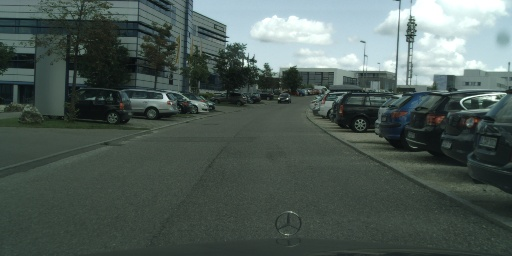
\includegraphics[width=0.25\textwidth]{figures/ulm_000088_000019_leftImg8bit.jpg}
    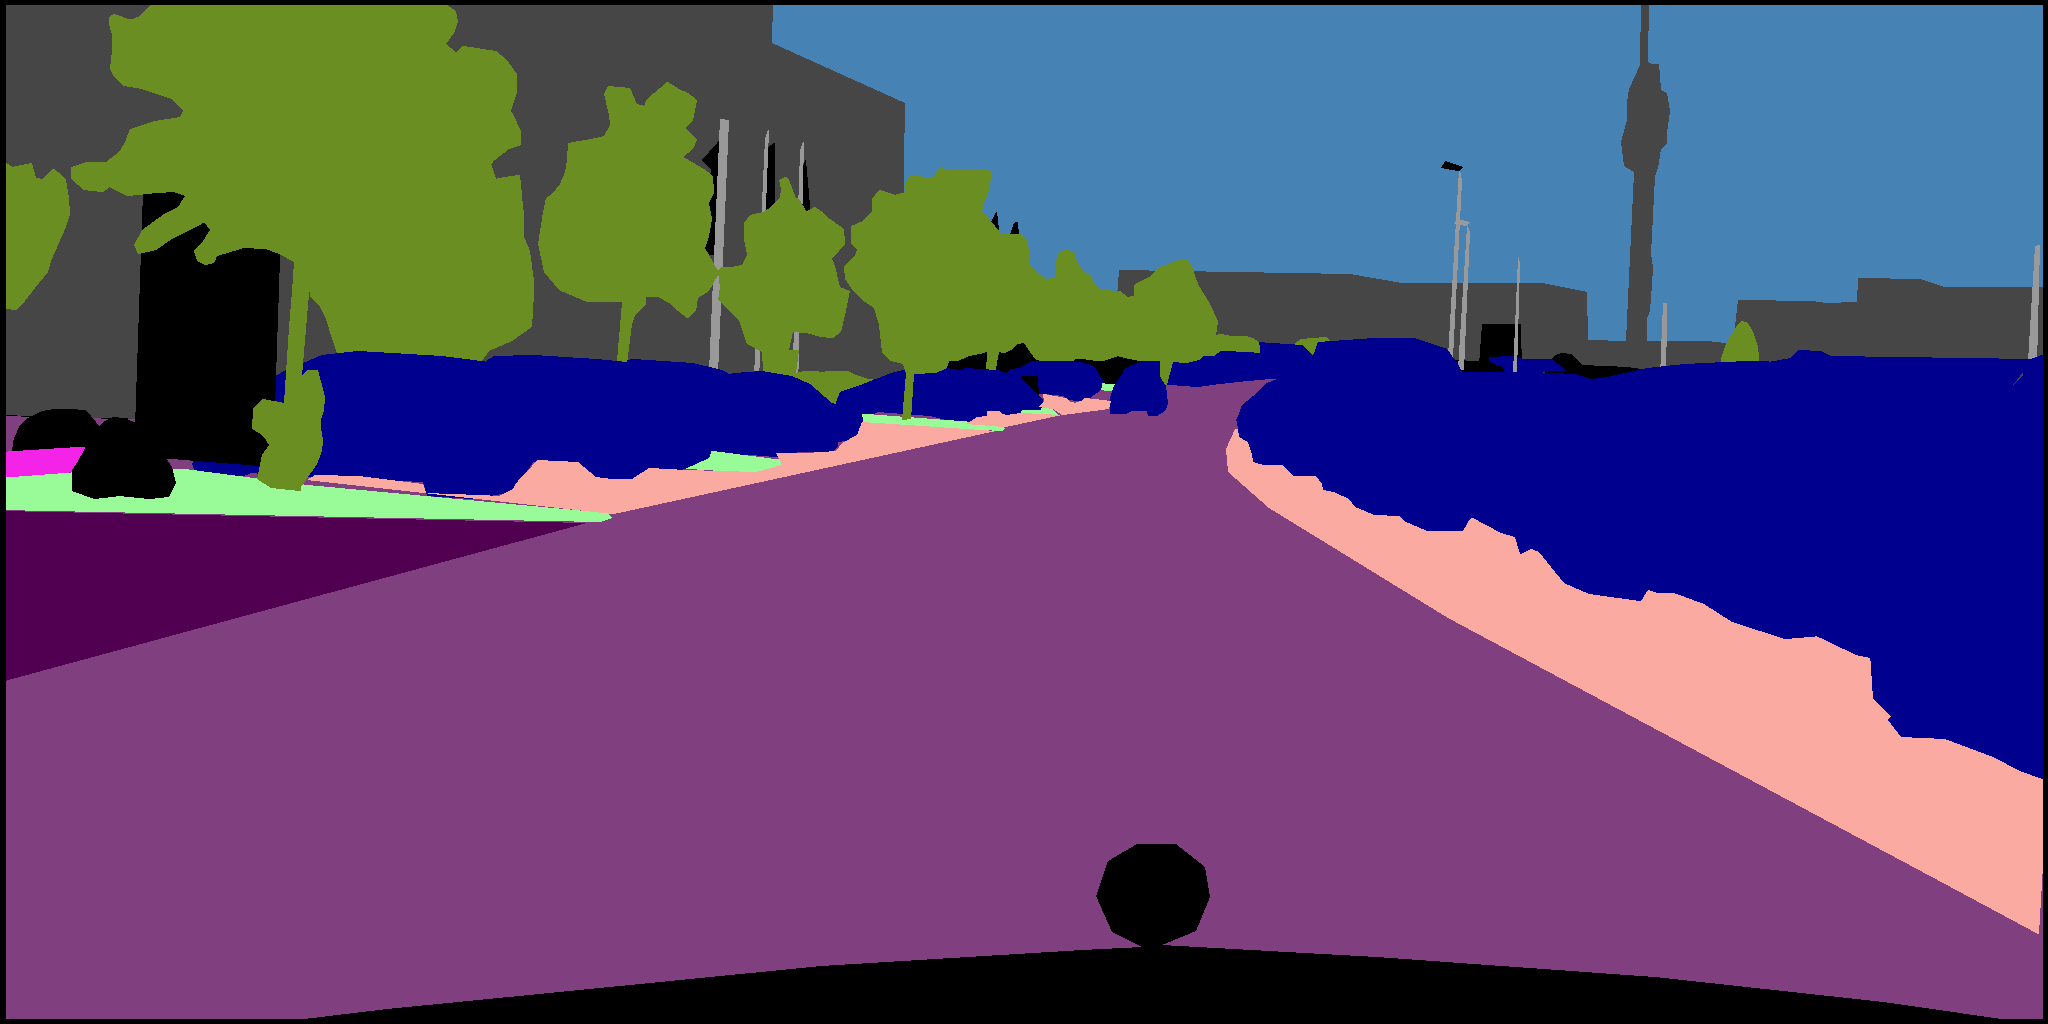
\includegraphics[width=0.25\textwidth]{figures/ulm_000088_000019_gtFine_color.png}
    \caption{Sample pair of images from the CITYSCAPES data set.}
    \label{fig:cityscapes}
\end{figure}
\textbf{GTA5} \cite{richter2016playing} is a synthetic dataset consisting of 24966 photo-realistic synthetic images with precise pixel-level semantic annotations. I went through the dataset and chose 16786 labelled images for training.
\begin{figure}[H]
    \centering
    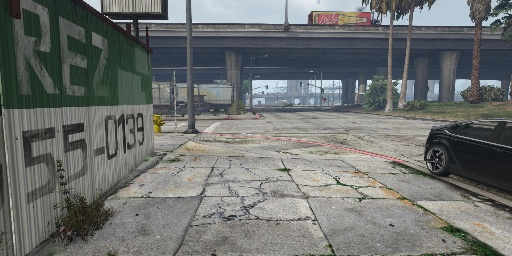
\includegraphics[width=0.25\textwidth]{figures/068_02196.jpg}
    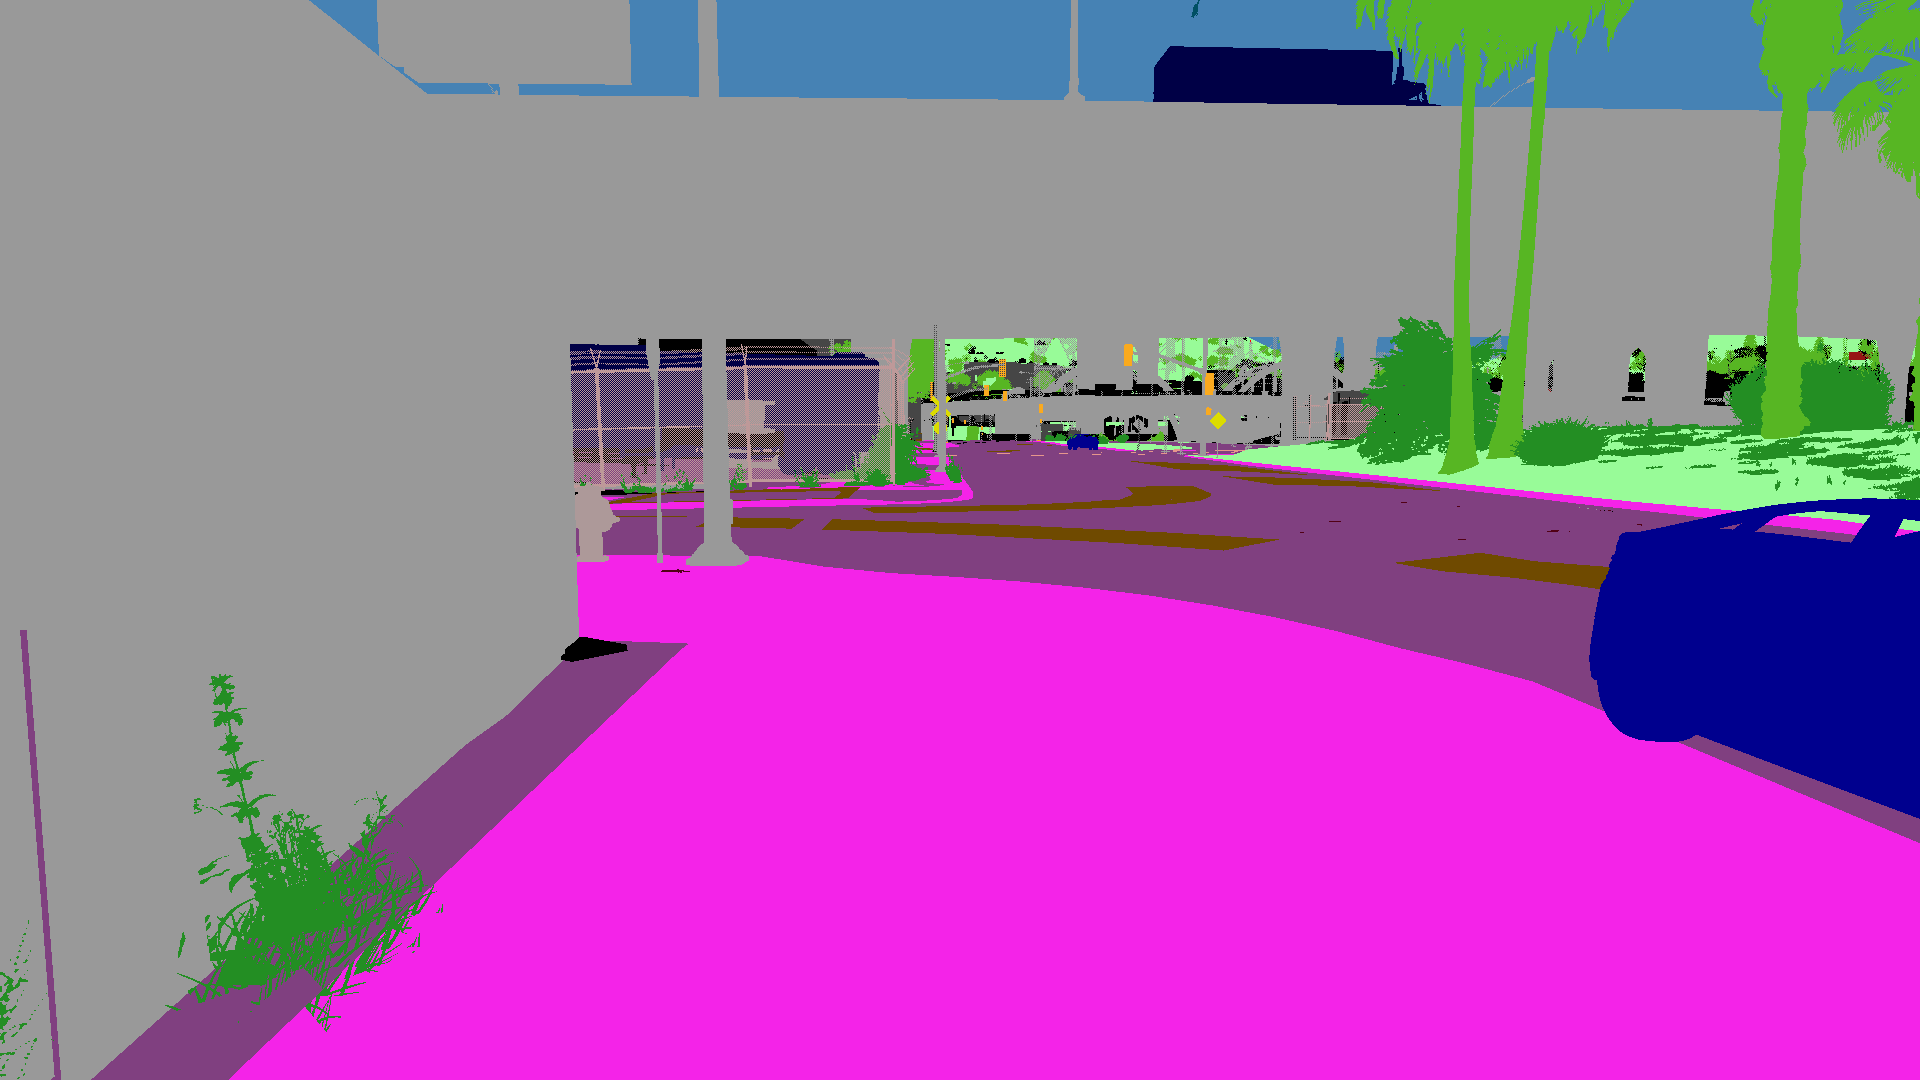
\includegraphics[width=0.25\textwidth]{figures/068_02196.png}
    \caption{Sample pair of images from the GTA5 data set. As can be noticed, the car is driving on a sidewalk, and scenes like this are very common in the GTA5 dataset. Worried that this might lead to a significant domain gap unresolvable by aligning styles, I went through the dataset and excluded them from our training set.}
    \label{fig:GTA5}
\end{figure}

\section{Models}
\subsection{Basic CycleGAN\cite{zhu2017unpaired}}
\begin{figure}[H]
    \centering
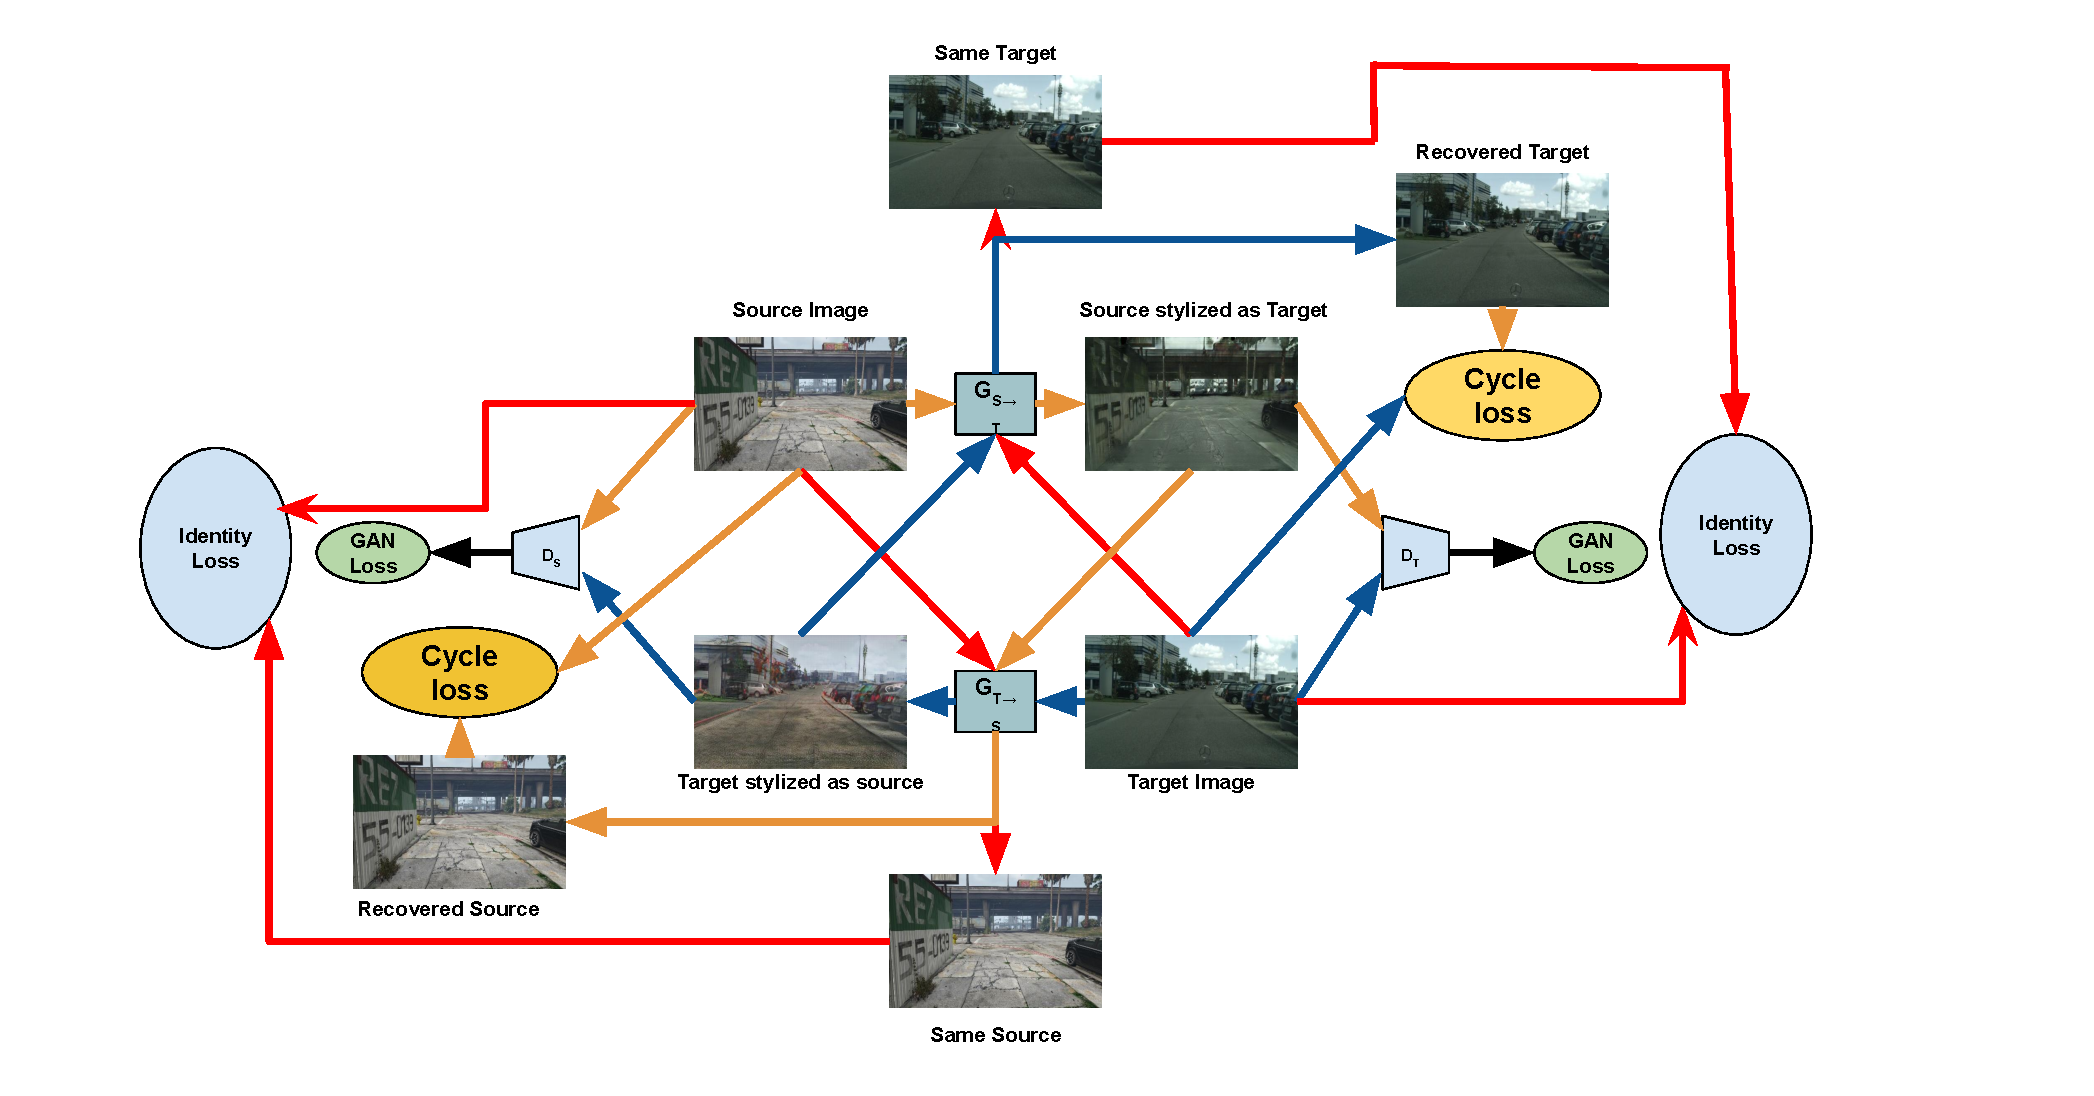
\includegraphics[width=0.7\textwidth]{figures/cygan.pdf}
\end{figure}
I added a classifier to preserve contents(cars, buildings) during domain transfer
\subsection{Backprop from classifier to generators}
\begin{figure}[H]
    \centering
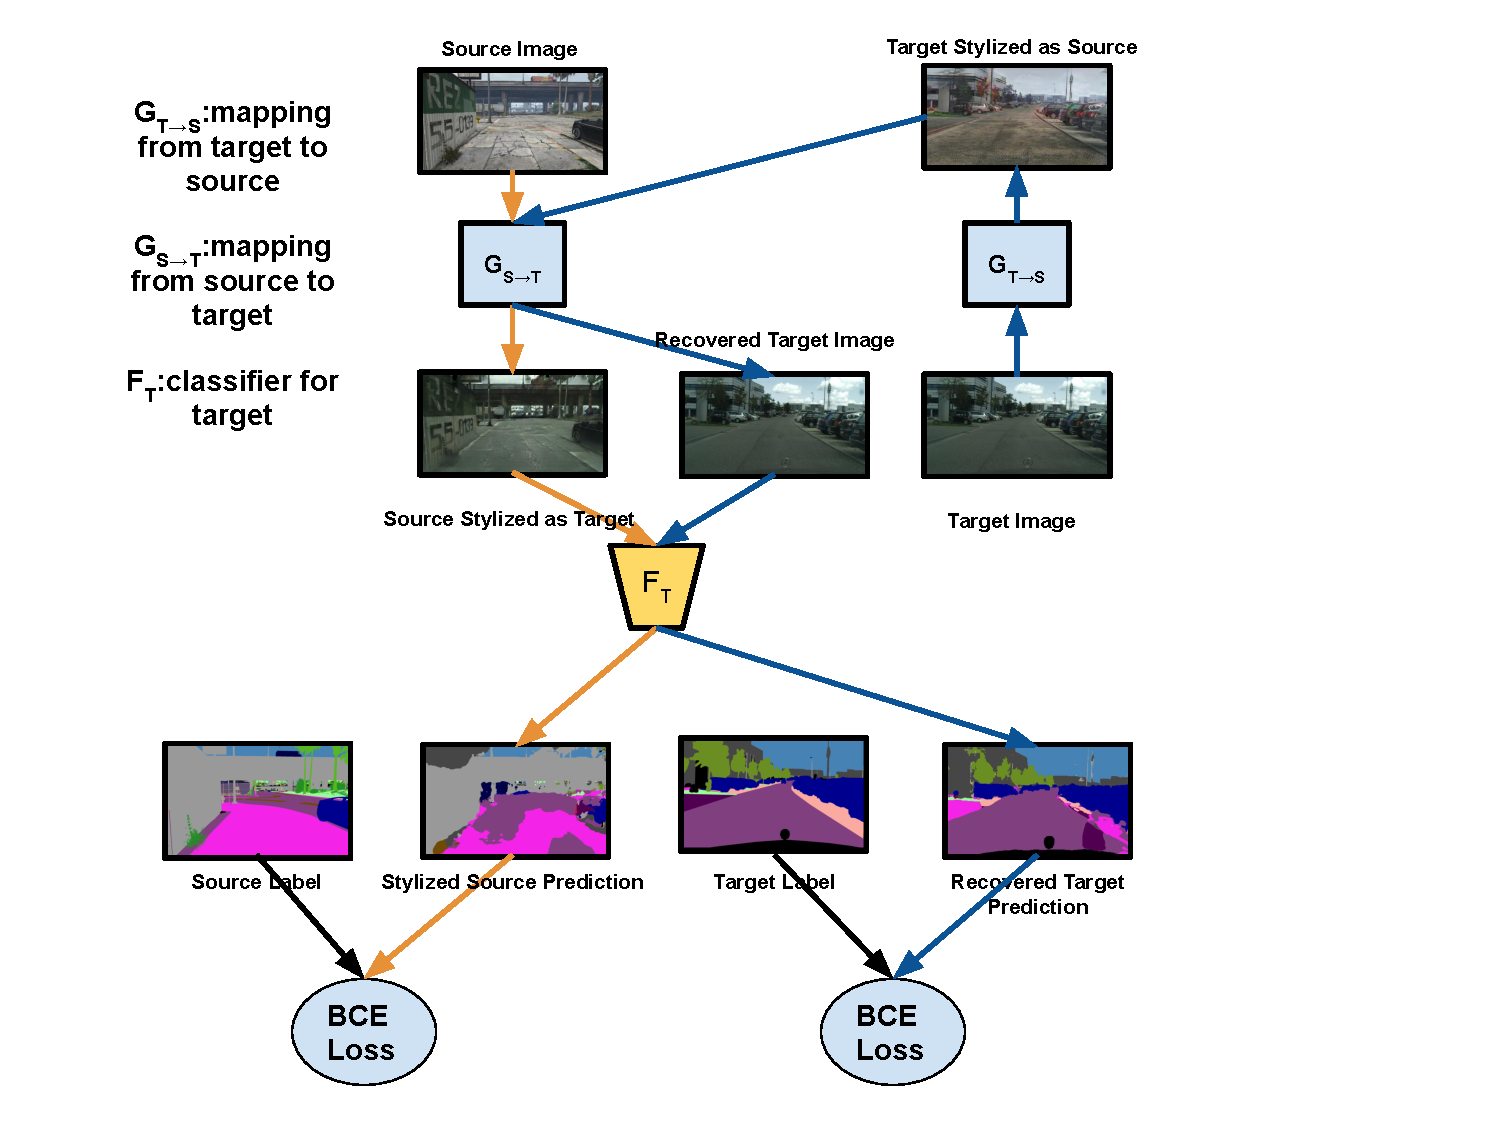
\includegraphics[width=0.7\textwidth]{figures/f_g.pdf}
\end{figure}

\subsection{Training Classifier}
\begin{figure}[H]
    \centering
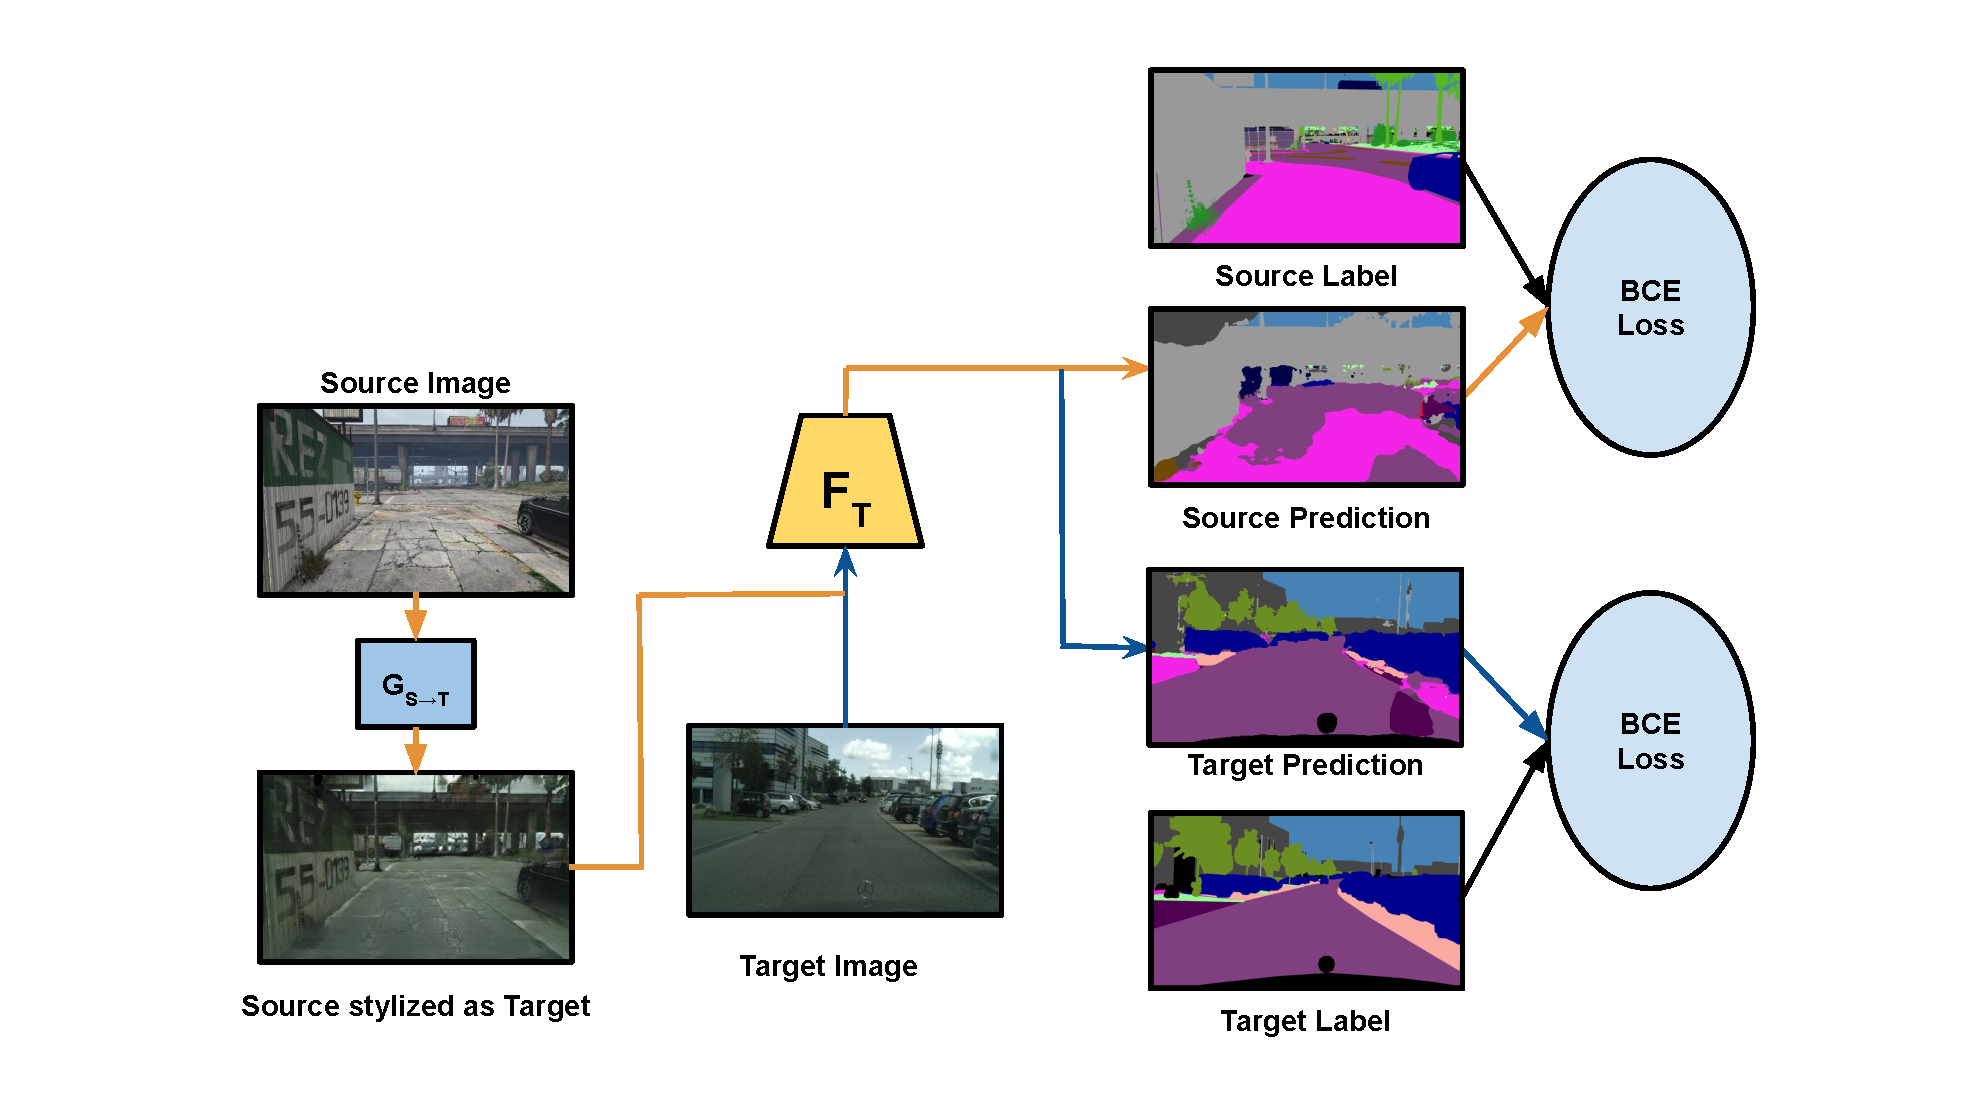
\includegraphics[width=0.7\textwidth]{figures/c_t.pdf}
\end{figure}

\section{Notations}
$X_S: $ Input from the source domain (GTA5).\\
$X_{SasT}: $ Input stylized as the target style (GTA5). This notation is introduced when the parameters of the $G_{S\rightarrow T}:$ generators are not involved in back propogation. \\
$Y_S: $ Label from the source domain. \\
$X_T: $ Input from the target domain (CITYSCAPES).\\
$Y_T: $ Input from the target domain.\\
$F_T: $ Classifier for the target domain.\\
$G_{S\rightarrow T}: $ Mapping from the source domain to the target.\\
$G_{T\rightarrow S}: $ Mapping from the target domain to the source.\\
$D_S:$ Discriminator for the source domain.\\
$D_T:$ Discriminator for the target domain.\\
$CE(X, Y, F_T): = -\mathcal{L}_{(x,y) \in (X,Y)}{[\sum_{k=1}^{K} \mathbbm{1}_{[y=k]} \log{[\sigma (F_T^{k}(x))]} ]}$ cross entropy loss, X and Y are the input and the label, $\sigma$ is the softmax function.
\section{Loss Functions}
The model learns mappings from the source domain to the target and the target to the source simultaneously. It is trained to produce samples that fools the discriminators in both domains.\\
$\mathcal{L}_{GAN}(G_{S\rightarrow T}, X_S, D_S, D_T) = \E_{ x_s\in X_S}{[\log{D_S(x_s)}+\log{[1-D_T(G_{S\rightarrow T}(x_s))]}]}$ \\
$\mathcal{L}_{GAN}(G_{T\rightarrow S}, X_T, D_S, D_T) = \E_{x_t\in X_T}{[\log{D_T(x_t)}+\log{[1-D_S(G_{T\rightarrow S}(x_t))]}]}$ \\\\
The model learns to preserve contents through the cycle consistency loss and segmentation loss.\\
$\mathcal{L}_{Cyc}(G_{S\rightarrow T},G_{T\rightarrow S}, X_S, X_T) = \E_{ x_s\in X_S, x_t\in X_T}{[{\left\lVert G_{T\rightarrow S}(G_{S\rightarrow T}(x_s)) -x_s \right\rVert}_1 + {\left\lVert G_{S\rightarrow T}(G_{T\rightarrow S}(x_t)) -x_t \right\rVert}_1]}$ \\
$\mathcal{L}_{G_{sem}}(G_{S\rightarrow T}, X_S, F_T, Y_S) = \E_{ (x_s, y_s)\in (X_S, Y_S)} {[CE(F_T(G_{S\rightarrow T}(x_s)), y_s)]}$\\
$\mathcal{L}_{G_{sem}}(G_{S\rightarrow T}, G_{T\rightarrow S}, X_T, F_T, Y_T) = \E_{ (x_t, y_t)\in (X_T, Y_T)} {[CE(F_T(G_{S\rightarrow T}(G_{T\rightarrow S}(x_t))),y_t)}]$\\\\
The classifier is trained on paired target data as well as paired source data stylized as target.\\
$\mathcal{L}_{sem}( X_{SasT}, X_T, Y_S, Y_T, F_T) = \E_{ (x_{sast}, y_s)\in (X_{SasT}, Y_S), (x_t, y_t)\in (X_T, Y_T)}{[CE(F_T(x_{sast}),y_s)+CE(F_T(x_t), y_t)]}$\\\\
The overall cycleGAN training loss is:\\
\begin{align*}
\mathcal{L}_{cycleGAN}(X_S, Y_S, X_T, Y_T, F_T, G_{S\rightarrow T}, G_{T\rightarrow S}, D_S, D_T) =  \mathcal{L}_{GAN}(G_{S\rightarrow T}, X_S, D_S, D_T)  + \mathcal{L}_{GAN}(G_{T\rightarrow S}, X_T, D_S, D_T) \\ + \mathcal{L}_{Cyc}(G_{S\rightarrow T},G_{T\rightarrow S}, X_S, X_T) + \mathcal{L}_{G_{sem}}(G_{S\rightarrow T}, X_S, F_T, Y_S) \\ +  \mathcal{L}_{G_{sem}}(G_{S\rightarrow T}, G_{T\rightarrow S}, X_T, F_T, Y_T) 
\end{align*}
\\Which corresponds to solving the optimization problem\\
\begin{align*}
\argmin_{G_{S\rightarrow T}, G_{T\rightarrow S}} \max_{D_S, D_T}  \mathcal{L}_{cycleGAN}(X_S, Y_S, X_T, Y_T, F_T, G_{S\rightarrow T}, G_{T\rightarrow S}, D_S, D_T) 
\end{align*}
\\The segmentation network is updated separately with:\\
\begin{align*}
\argmin_{F_T} \mathcal{L}_{sem}( X_{SasT}, X_T, Y_S, Y_T, F_T) 
\end{align*}

\section{Experiments}
\subsection{Changing percentages of real(target) data used in our model}
In this experiment, we kept the dataset size fixed, and only included paired data from both domains, changing the percentage each takes.\\
When the percentage of real data is 0\%, our classifier is only trained on data from the source domain(GTA5), and tested on CITYSCAPES validation set.\\
When the percentage of real data is 100\%, our classifier is only trained on data from the target domain(CITYSCAPES), and tested on CITYSCAPES validation set.\\
When the percentage is between 0 and 100\%, our classifier is trained end to end with CycleGAN that stylizes data from the source domain as the target.\\
The baseline is a classifier with the same architecture as ours, trained without style transfer.\\
\begin{figure}[H]
    \centering
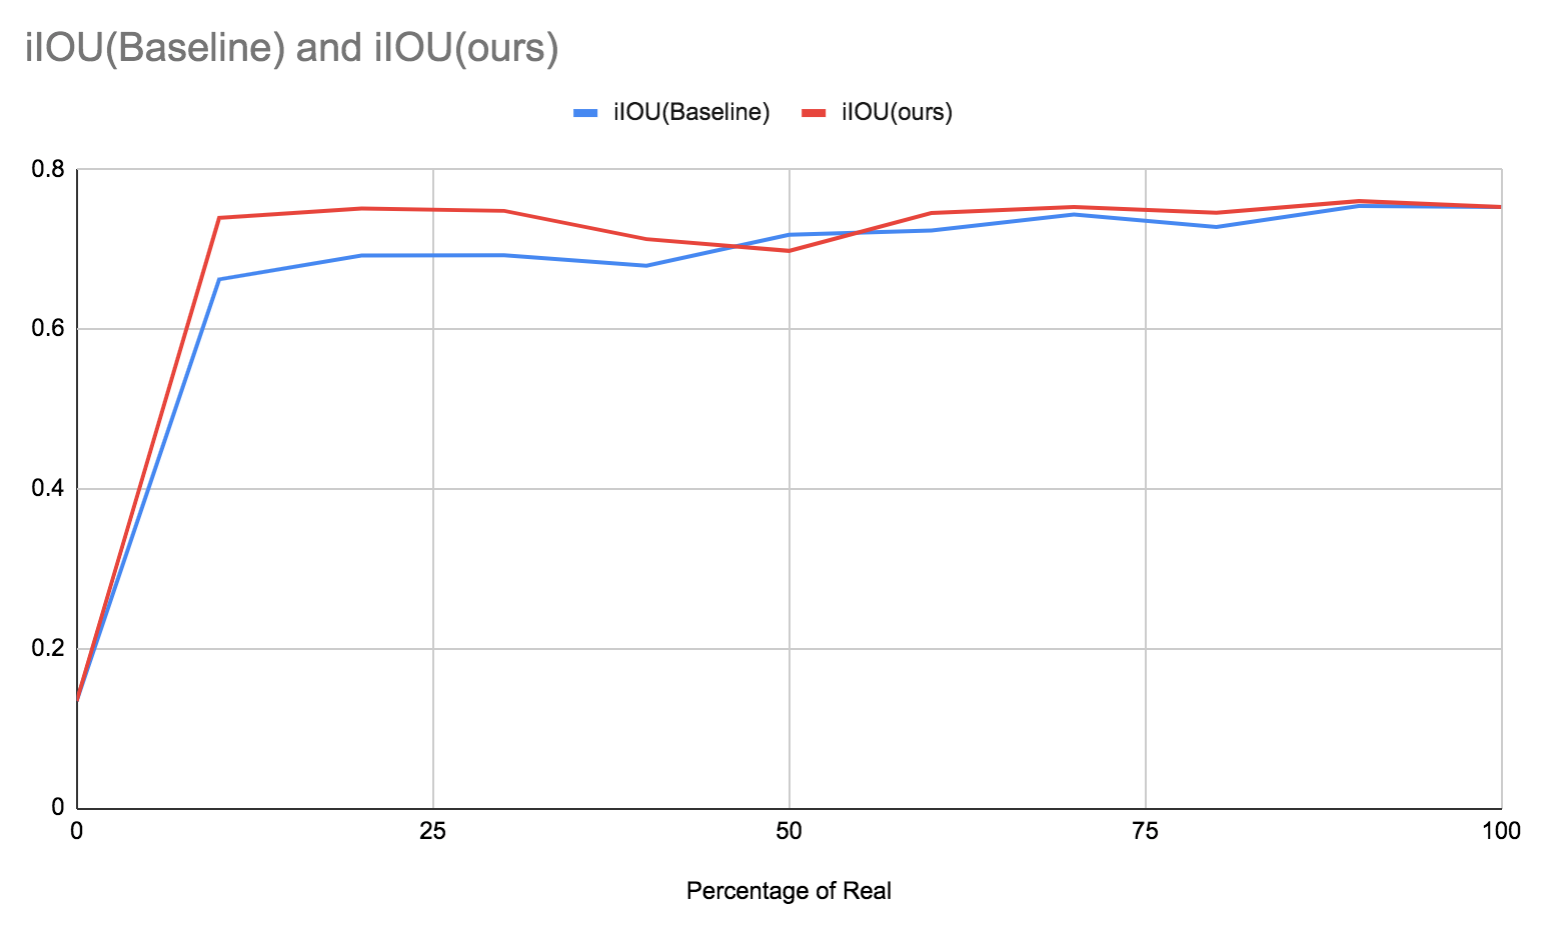
\includegraphics[width=0.7\textwidth]{figures/real_p.png}\\
\end{figure}

The evaluation metric used is weighted IOU. Our method achieved 75\% accuracy with 10\% of paired data from the target domain, but stops further improving as the percentage increases. Notice that the baseline reached \%75 accuracy when around 90\% of paired real data is used. But it's possible that the architecture for the classifier is too simple(U-Net) that it is not capable of learning more.\\

\begin{figure}[H]
    \centering
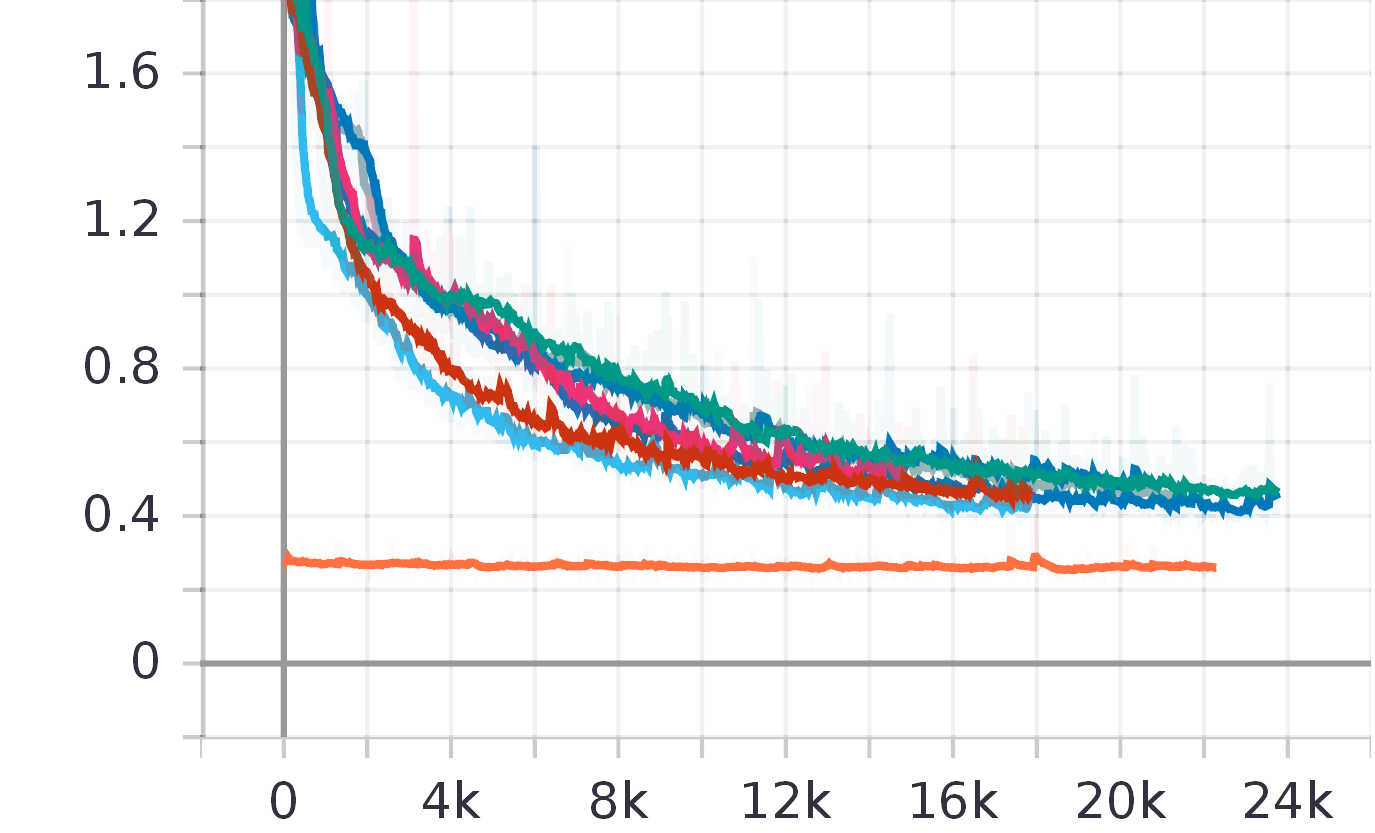
\includegraphics[width=0.7\textwidth]{figures/realx_base (1).png}\\
\caption{keeping the training dataset size fixed, varying percentage of paired data (10\% to 90\%) in CITYSCAPES + GTA5 stylized as CITYSCAPES to train the segmentation network. The orange line is the fully supervised model using only CITYSCAPES pairs (oracle).  It seems like style transfer might have negative effects.}
\end{figure}


\begin{figure}[H]
    \centering
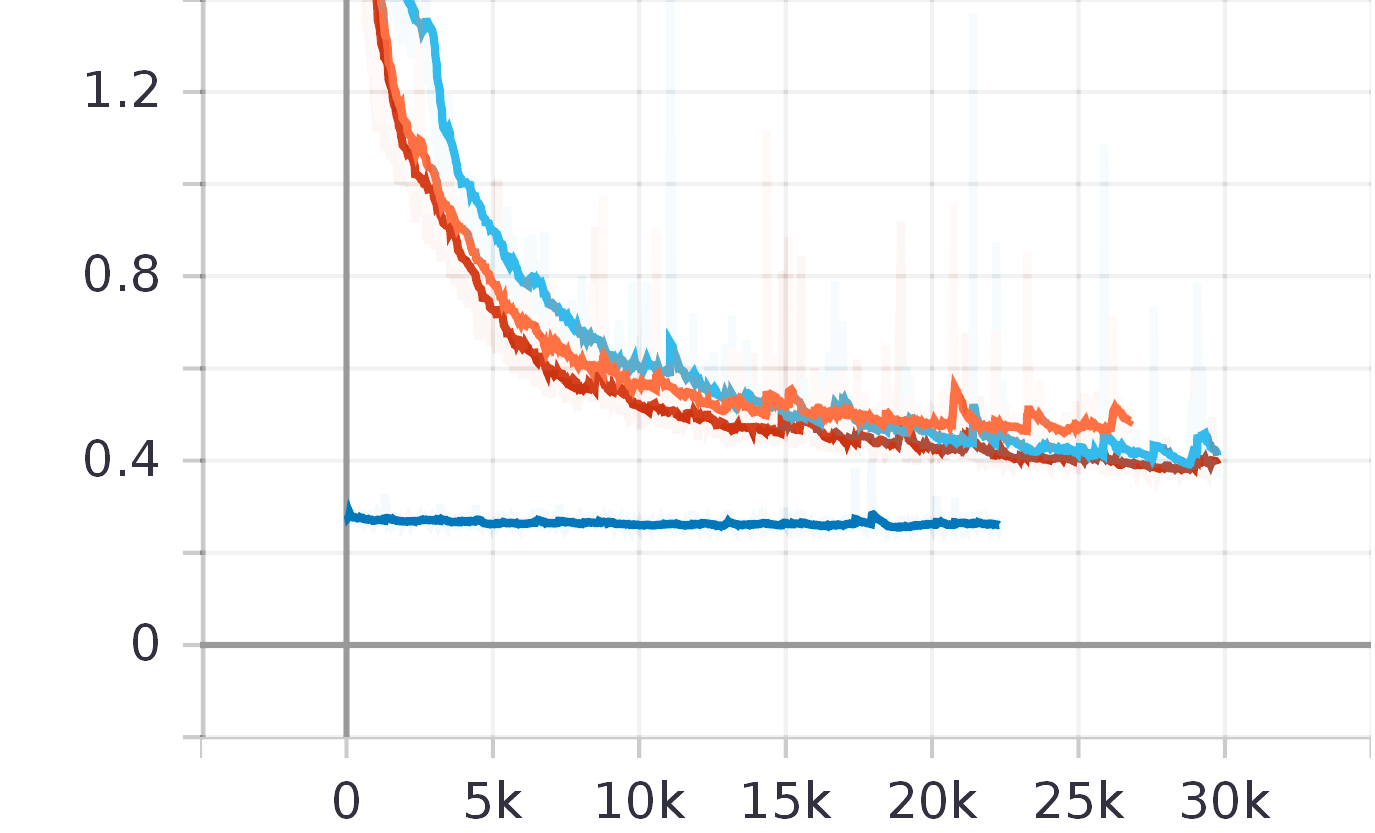
\includegraphics[width=0.7\textwidth]{figures/real100_and_syn (1).png}\\
\caption{using all the paired data in CITYSCAPES + varying percentage of GTA5 (10\%, 20\%, 50\% of total) stylized as CITYSCAPES paired data to train the segmentation network. The blue line is the fully supervised model using only CITYSCAPES pairs (oracle) It seems like style transfer might have negative effects.}
\end{figure}

\section*{new approach}
In the first stage, train a segmentation network with GTA5 pairs to use as auxiliary loss for cycleGAN training. This should be replaced by some pre-trained network, i.e. a VGG.\\
In the second stage, train the normal cycleGAN, obtain a generator G that maps from GTA5 to CITYSCAPES and a discriminator $D_T$ that tells if an image is from the target domain .\\
In the third stage, train a segmentation network $F_T$ using stylized GTA5 pairs.\\
In the fourth stage, train $F_T$ end to end with G, discriminator $D_T$ and $D_F$. $D_T$ tells if an image is from the target domain, in our case CITYSCAPES. $D_F$ tells if a semantic map looks real, and we hope that adversarial training with $D_F$ will force $F_T$ to output realistic semantic maps for unsupervised domain CITYSCAPES.

\begin{figure}[H]
    \centering
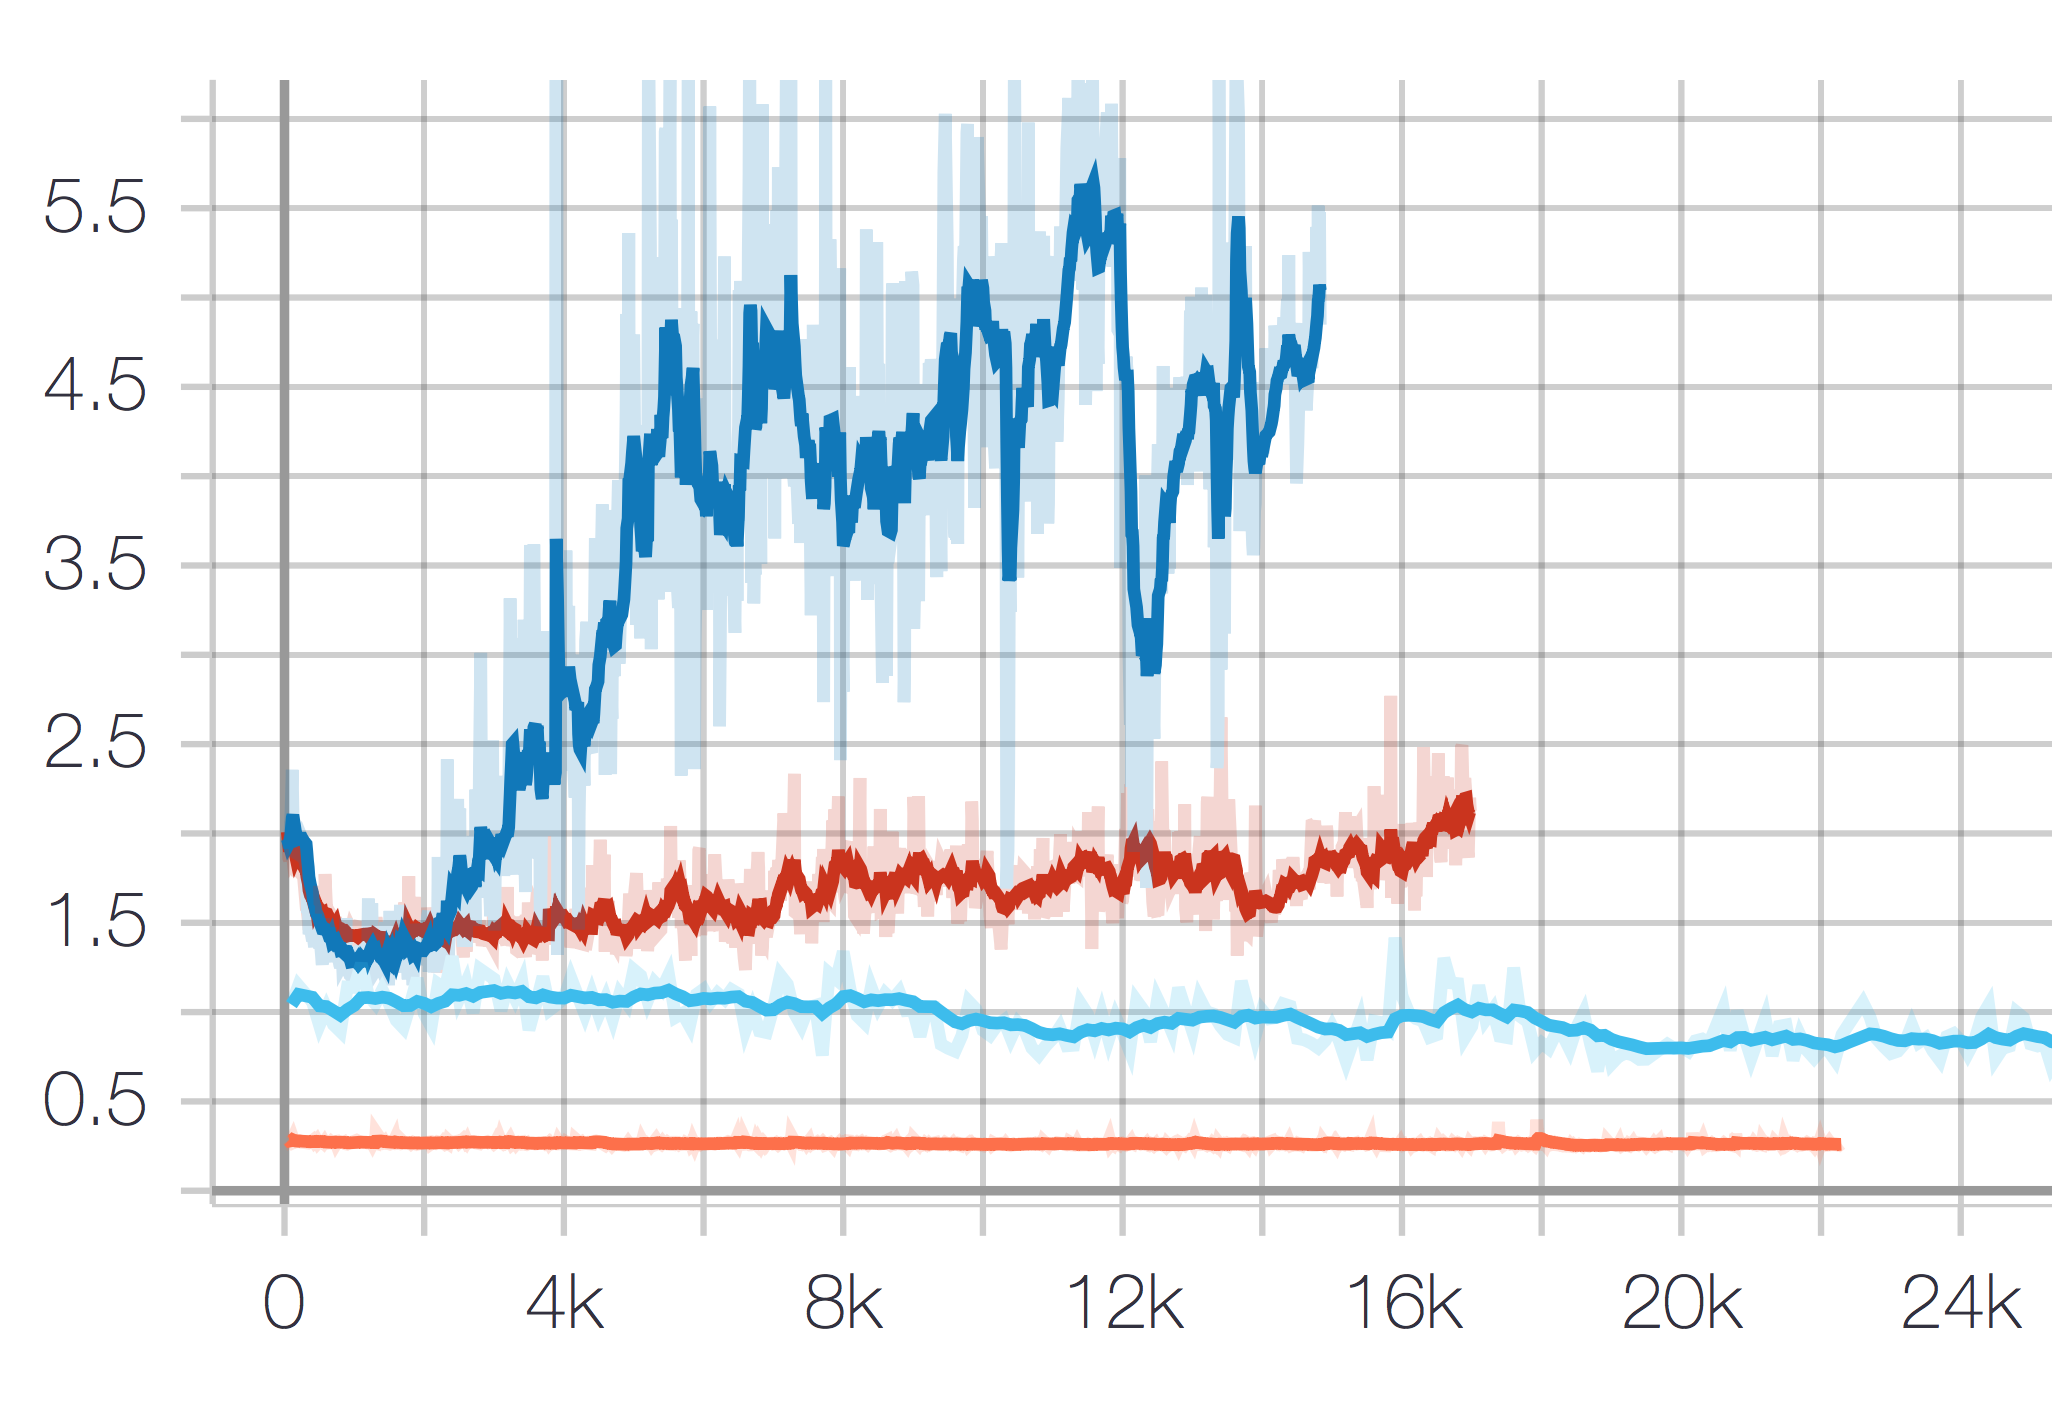
\includegraphics[width=0.7\textwidth]{figures/syn_tran_base.png}\\
\caption{validation error of different models. newly proposed model- sky blue, source only- dark blue, stylized GTA5- red, and orange is the oracle model using all CITYSCAPES pairs.}
\end{figure}


\section*{TODOs}
change baseline to deeplab v3 + resnet and retrain\\
train with current size cityscapes with full GTA5 and evaluate the performance.\\
train with full size cityscapes with cleaned GTA5 and evaluate the performance.\\
train with full size cityscapes with full GTA5 and evaluate the performance.\\
train Cycada \cite{hoffman2017cycada} and compare\\
train Fcns in the wild \cite{hoffman2016fcns} and compare\\
train \cite{tsai2018learning} and compare\\
train \cite{Chen_2018_CVPR} and compare

\section*{Issues}
Adjust the weights on loss for segmenting stylized images when increasing the percentage of source data used.\\
The sample is unbalanced(most instances are road and sky), adjust the weights for different class?\\
training segmentation network and generators end to end might not work? keep segmen network fixed, train cygan, cygan converges and fixed, train segmen?
\bibliography{summary}
\bibliographystyle{plain}

\end{document}

